%\usepackage{float}
\documentclass{article}
\usepackage{hyperref}
\usepackage{graphicx} % Required for inserting images
\usepackage[english]{babel}
%\usepackage{titlesec}


\title{ANALYSIS OF COVID-19 CHEST X-RAYS: Report 2: Modeling Report}
\author{Saniya Arfin, Yvonne Breitenbach, Alexandru Buzgan}
\date{May 2025}

\begin{document}

\maketitle

\tableofcontents

\newpage 

\section{Introduction}
\begin{itemize}
    \item What kind of machine learning problem is your project like? (classification, regression, clustering, etc)
    \item What task does your project relate to? (fraud detection, facial recognition, sentiment analysis, etc)?
    \item ...
\end{itemize}

\section{Methods}

\subsection{Prepare Data for Modelling}
Just a summary of the points we found out in report 1, that we have to do with the images. Maybe we need a different order.
\begin{itemize}
    \item convert to grayscale
    \item Contrast Enhancement with CLAHE
    \item resize the masks and combine them with images
    \item Pixel Value Normalization
    \item Label Encoding: Convert categorical class labels (e.g., COVID, Normal, Pneumonia, Lung Opacity) into numerical format for compatibility with machine learning algorithms.
    \item Dataset Splitting: Partition the dataset into training, validation, and test subsets to enable robust model evaluation and prevent data leakage.
    \item Address Class Imbalance: Since the distribution between the classes is not balanced (for example Viral Pneumonia images are far less numerous than the Normal images) we have to address this problem before the training stage. Appropriate strategies will be applied, such as:
    \begin{itemize}
        \item Class weighting during model training
        \item Oversampling/undersampling
        \item Data augmentation for minority classes
    \end{itemize}
    \item This ensures the model does not become biased toward the majority classes and maintains fair performance across all categories.
\end{itemize}

Maybe we need two different data preparation pipelins: one for the machine learning models and another one for the deep learning models

\subsubsection{Prepare Data for Machine Learning Models}


\subsubsection{Prepare Data for Deep Learning Models}

\subsection{Metrics to Evaluate the Model Results}

Idea is to determine metric which we want to use to evaluate the performance of all our tested models.
\begin{itemize}
    \item What is the main performance metric used to compare your models? Why
    this one?
    \item Did you use other qualitative or quantitative performance metrics? If yes,
    detail it.
\end{itemize}


\subsection{Used Models: Machine Learning}
Some ideas, questions for this chapter:

\begin{itemize}
    \item What algorithms have you tried?
    \item Describe which one(s) you selected and why?
    \item Did you use parameter optimization techniques such as Grid Search and Cross Validation?
    \item Have you tested advanced models? Bagging, Boosting, Deep Learning… Why?
\end{itemize}

\subsubsection{? Decision Trees ?}
just a random example
\subsubsection{? Random Forst ?}
just a random example

\subsubsection{Used Models: Optimized Machine Learning}
Romain mentioned something like that, that there is a library for that.

\subsection{Used Models: Deep Learning}

\subsubsection{? Model 1 ?}
\subsubsection{? Model 2 ?}

\subsection{Transfer Learning}
we have to find out more about that, but Romain mentioned it.

\section{Results}
Some ideas, questions for this section:

\begin{itemize}
    \item Have you analyzed the errors in your model?
    \item Did this contribute to his improvement? If yes, describe.
    \item Have you used interpretability techniques such as SHAP, LIME, Skater… (Grad-CAM for Deep Learning…)
    \item What has (or not) generated a significant improvement in your performance?
\end{itemize}



\subsection{Results ? Decision Trees ?}
just a random example

\subsection{Results ? Random Forst ?}
just a random example

\section{Conclusion}
Overall Conclusion
Which model performed best
What worked, what did not work? Why?

\section{Example include image and table}

Put images you want to include to this report in the subfolder: figures\_report\_2 and use relative paths inside this report.
Upload them on git aswell.

\begin{figure}[h!] % the [h!] helps force it "here"
    \centering
    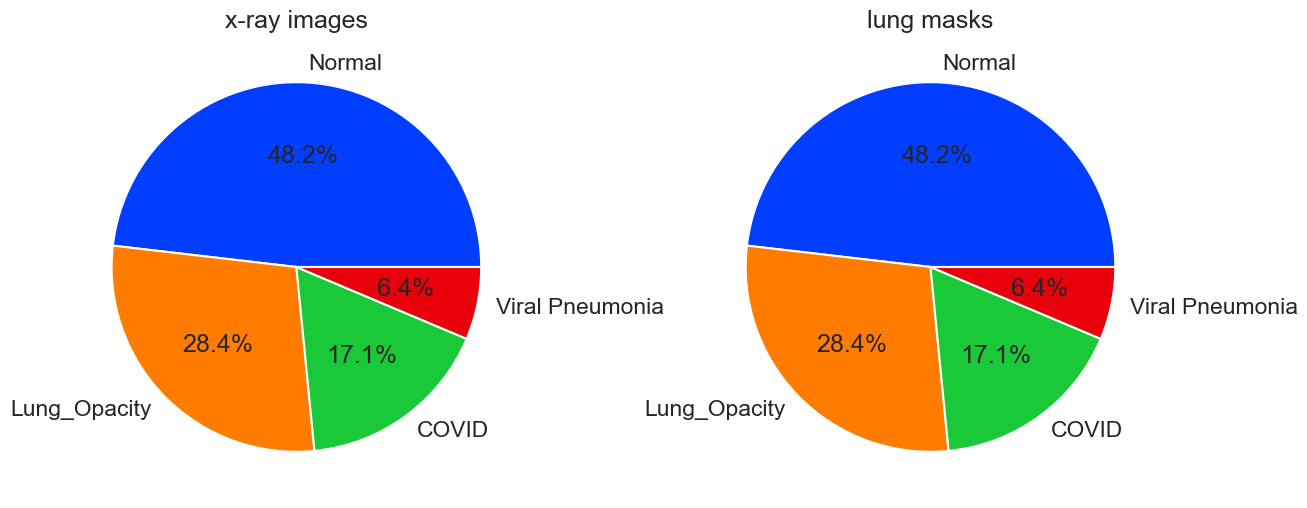
\includegraphics[width=1.0\linewidth]{../figures/figures_report_2/classes.png}
    \caption{Examples of image}
    \label{fig:example_image}
\end{figure}

Figure \ref{fig:example_image} shows ...


\begin{table}[h]
    \centering
    \begin{tabular}{|c|c|c|}
        \hline
        \textbf{X} & \textbf{Y} & \textbf{Z} \\ \hline
        1 & 2 & 3 \\ \hline
        4 & 5 &  \\ \hline \hline
        6 &  & 7 \\ \hline
    \end{tabular}
    \caption{Example of table}
    \label{tab:example_table}
\end{table}

Table \ref{tab:example_table} shows \dots

\end{document}
